%! TEX program = pdflatex

\documentclass[oneside,solution]{tmpl}

\usepackage[utf8]{inputenc}
\usepackage[english,ukrainian]{babel}

\title{Домашня робота}
\author{Захаров Дмитро}
\studentID{МП-31}
\instructor{Ігнатович С.Ю.}
\date{\today}
\duedate{23:59 15 квітня, 2024}
\assignno{5}
\semester{Весняний семестр 2024}
\mainproblem{Фазові портрети нелінійних двовимірних систем.}

\begin{document}

\maketitle

% \startsolution[print]

\problem{Синуси.}

\textbf{Умова.} Розглянемо систему
\begin{equation}
    \begin{cases}
        \dot{x}_1 = \sin x_1 \\
        \dot{x}_2 = \sin x_2
    \end{cases}
\end{equation}

Знайдіть її точки спокою і лінеаризацію системи в цих точках. Спробуйте намалювати (глобальний) фазовий портрет цієї системи. Перевірте себе за допомогою програми (методу \texttt{streamplot}). 

\textbf{Розв'язок.} Векторне поле праворуч має вигляд:
\begin{equation}
    \boldsymbol{f}(x_1,x_2) = (\sin x_1, \sin x_2)
\end{equation}

Таким чином, можемо знайти Якобіан:
\begin{equation}
    \boldsymbol{J} \triangleq \frac{\partial \boldsymbol{f}}{\partial \mathbf{x}} = \begin{bmatrix}
        \frac{\partial f_1}{\partial x_1} & \frac{\partial f_1}{\partial x_2} \\
        \frac{\partial f_2}{\partial x_1} & \frac{\partial f_2}{\partial x_2}
    \end{bmatrix} = \begin{bmatrix}
        \cos x_1 & 0 \\ 0 & \cos x_2
    \end{bmatrix}
\end{equation}

Знайдемо точки спокою: тобто множину точок, для яких $\boldsymbol{f}$ приймає нульове значення. Маємо:
\begin{equation}
    \begin{cases}
        \sin x_1 = 0 \\ 
        \sin x_2 = 0
    \end{cases} \implies (x_1,x_2) = (\pi n, \pi k), \; n,k \in \mathbb{Z}
\end{equation}

Тобто, множина точок спокою -- це квадратна решітка з точок з шириною клітинки $\pi$, що проходить через $(0,0)$. Для класифікації точок, нам потрібно обчислити Якобіан в цих точках:
\begin{equation}
    \boldsymbol{J}(\pi n, \pi k) = \begin{bmatrix}
        (-1)^n & 0 \\ 0 & (-1)^k
    \end{bmatrix} = \text{diag} \{(-1)^n, (-1)^k\}
\end{equation}

Звідси характеристичний поліном $\chi_{J}(\lambda) = (\lambda - (-1)^n)(\lambda - (-1)^k)$ і спектр $\sigma(\boldsymbol{J}(\pi n, \pi k)) = \{(-1)^n, (-1)^k\}$. В залежності від парностей $n,k$ можливо 4 випадки:

\textbf{Випадок 1. $n,k$ -- парні} Тоді спектр складається з єдиного власного значення $\lambda=1$ кратності $2$. Це відповідає фазовому портрету множини прямих, що проходять через $(\pi n, \pi k)$, причому траєкторія виходить з точок, що відповідає нестійкій точці.

\textbf{Випадок 2. $n,k$ -- непарні.} Спектр складається з єдиного власного значення $\lambda = -1$ кратності $2$ -- це також відповідає множині прямих, але траєкторія входить в точку, тобто вона є стійкою.

\textbf{Випадок 3. $n$ -- парне, $k$ -- непарне.} Спектр складається з двох власних значень $\{-1,1\}$. Оскільки обидва значення є дійсними і протилежними за знаком, то перед нами сідло.

\textbf{Випадок 4. $n$ -- непарне, $k$ -- парне.} Як і у випадку 3, перед нами сідло.

Отже, яку поведінку ми очікуємо? По-перше, траєкторії мають сходитися до точок виду $((2p+1)\pi,(2q+1)n), \; p,q\in\mathbb{Z}$. Також, вони будуть візуально ``виходити'' з точок виду $(2p\pi, 2q\pi)$ (такі собі ``джерела'') і проходити ``повз'' точок $((2p+1)\pi, 2q\pi)$ та $(2p\pi, (2q+1)\pi)$ по траєкторіям, що схожі на гіперболи. 

Як і було запропоновано в умові, перевіримо гіпотезу за допомогою \textit{Python}. Запустимо наступну програму:
\begin{lstlisting}[language=Python]
import numpy as np
import matplotlib.pyplot as plt
from matplotlib.ticker import (AutoMinorLocator, MultipleLocator)

if __name__ == '__main__':    
    # Defining the matplotlib figure and axis.
    fig = plt.figure(figsize=(7, 7))
    ax = fig.add_subplot()
    
    # Change major ticks to show every pi.
    ax.xaxis.set_major_locator(MultipleLocator(np.pi))
    ax.yaxis.set_major_locator(MultipleLocator(np.pi))
    
    # Change minor ticks to show every pi/2.
    ax.xaxis.set_minor_locator(AutoMinorLocator(np.pi / 2))
    ax.yaxis.set_minor_locator(AutoMinorLocator(np.pi / 2))
    
    # Turn grid on for both major and minor ticks and style minor slightly
    # differently.
    ax.grid(which='major', color='#CCCCCC', linestyle='--')
    ax.grid(which='minor', color='#CCCCCC', linestyle=':')
    ax.set_aspect('equal')

    # Defining the vector field
    def f(x,y):
        return np.sin(x), np.sin(y)
    
    x = np.linspace(-1.75*np.pi, 1.75*np.pi, 100)  
    y = np.linspace(-1.75*np.pi, 1.75*np.pi, 100)  
    xx, yy = np.meshgrid(x, y)

    f1,f2 = f(xx, yy)	
    ax.streamplot(xx, yy, f1, f2, density=1.8, color='b')
    
    # Set high DPI and save the figure
    fig.set_dpi(300)
    fig.savefig(f'phase_portrait.png')
\end{lstlisting}

Результат зображено на Рисунку \ref{fig:problem_1}. Дійсно, малюнок відповідає нашій гіпотезі.

\begin{figure}
\begin{tabular}{cc}
  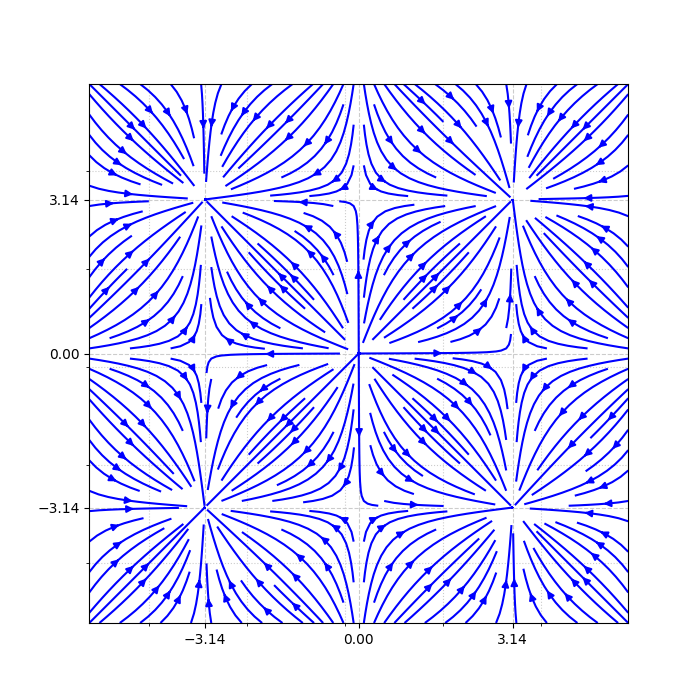
\includegraphics[width=0.5\textwidth]{images/hw_5/phase_portrait_1.png} &   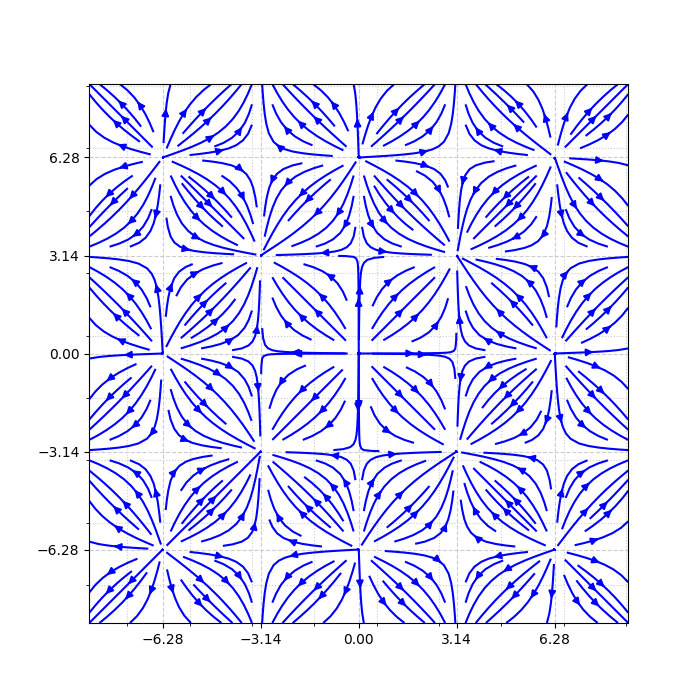
\includegraphics[width=0.5\textwidth]{images/hw_5/phase_portrait_2.png}
\end{tabular}
    \caption{Фазовий портрет для задачі 1. Ліворуч -- для області значень $(x,y) \in [-1.75\pi, +1.75\pi]^2$, праворуч -- для $(x,y) \in [-2.75\pi,+2.75\pi]^2$.}
    \label{fig:problem_1}
\end{figure}

\problem{Коливання без тертя.}

\textbf{Умова.} Розглянемо систему коливань маятника без тертя:
\begin{equation}
    \begin{cases}
        \dot{x}_1 = x_2 \\
        \dot{x}_2 = -\omega^2 \sin x_1
    \end{cases}
\end{equation}

Знайдіть точки спокою і лінеаризиацію системи в цих точках. Які висновки можна з цього зробити щодо фазового портрету вихідної системи в околі цих точок?

\textbf{Розв'язок.} Маємо векторне поле $\boldsymbol{f}(x_1,x_2) = (x_2,-\omega^2 \sin x_1)$. Точки спокою відповідають розв'язкам системи

\begin{equation}
    \begin{cases}
        x_2 = 0 \\
        -\omega^2 \sin x_1 = 0
    \end{cases} \implies (x_1, x_2) = (\pi n, 0), \; n \in \mathbb{Z}
\end{equation}

Для класифікації нам потрібно лінеаризувати систему. Для цього знайдемо Якобіан:
\begin{equation}
    \boldsymbol{J} \triangleq \frac{\partial\boldsymbol{f}}{\partial\mathbf{x}} = \begin{bmatrix}
        0 & 1 \\
        -\omega^2 \cos x_1 & 0
    \end{bmatrix}
\end{equation}

В точках спокою маємо:
\begin{equation}
    \boldsymbol{J}(\pi n, 0) = \begin{bmatrix}
        0 & 1 \\ \omega^2 (-1)^{n+1} & 0
    \end{bmatrix}
\end{equation}

Характеристичний поліном $\chi_J(\lambda) = \lambda^2 - \omega^2(-1)^{n+1}$. Отже, маємо два випадки.

\textbf{Випадок 1. $n$ -- парне.} Тоді $\lambda^2 = -\omega^2 \implies \lambda = \pm \omega i$ -- маємо два спряжених чисто комплексних значень. Це відповідає центру для лінеаризації $\dot{\mathbf{x}} = \boldsymbol{J}(2\pi k, 0)\mathbf{x}$. Хоча і інтуїтивно здається, що перед нами дійсно \textbf{центр}: випадок парних $n$ відповідає, наприклад, положенню математичного маятника у найнижчому положені (оскільки кут можна вказати з точністю до періода в $2\pi$, то звідси нескінченна кількість значень), проте чисто з аналізу спектру ми сказати щось конкретне не можемо. 

\textbf{Випадок 2. $n$ -- непарне.} Тоді $\lambda^2 = \omega^2 \implies \lambda = \pm \omega$ -- маємо два протилежних за знаком власних значень. Це відповідає \textbf{сідлу}, причому і для нелінійної системи також. Це теж достатньо логічно, оскільки якщо відхилити маятник на кут $\pi$, то це положення буде нестійким і маятник швидко почне відхилятися. 

Якщо зобразити портрет, то отримаємо Рисунок \ref{fig:no_friction}.

\begin{figure}
    \centering
    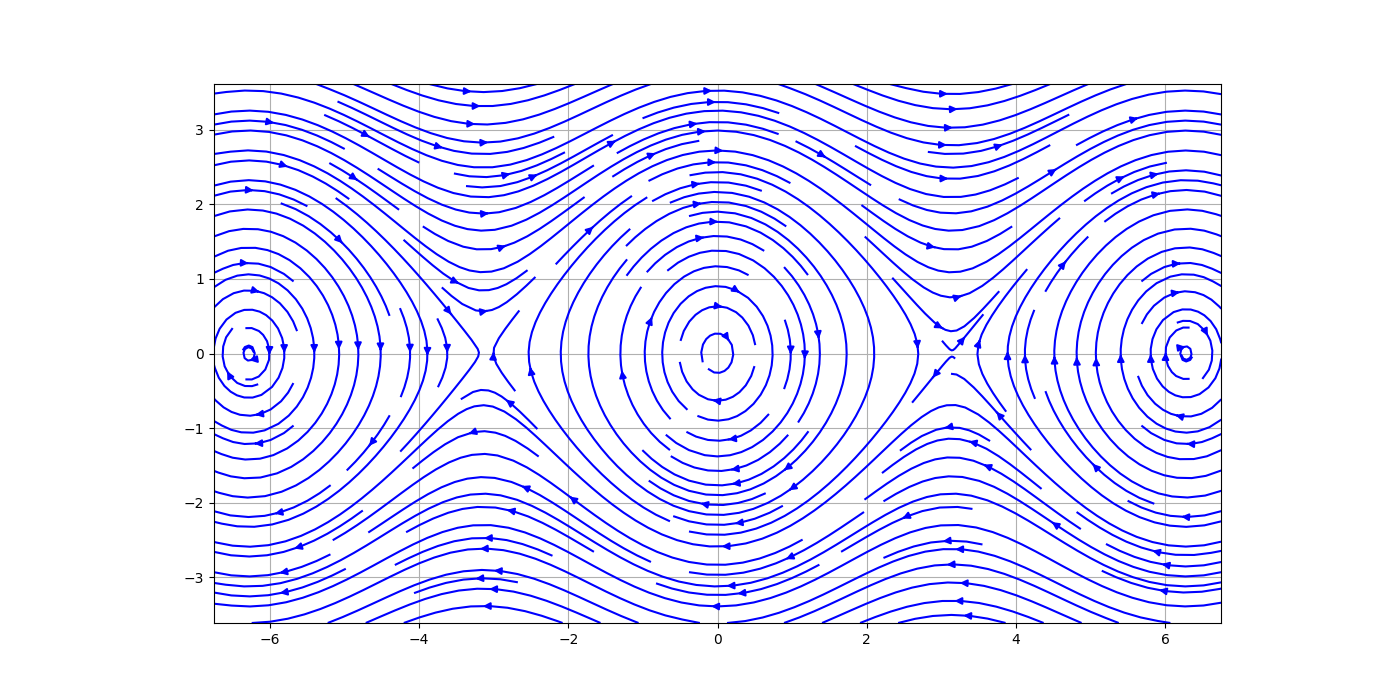
\includegraphics[width=\textwidth]{images/hw_5/no_friction_portrait.png}
    \caption{Фазовий портрет для системи з полем $\boldsymbol{f}(x_1,x_2)=(x_2,-\omega^2 \sin x_1)$. Область значень $(x,y) \in [-2.15\pi, 2.15\pi] \times [-1.15\pi, 1.15\pi]$}
    \label{fig:no_friction}
\end{figure}

\problem{Коливання з тертям.}

\textbf{Умова.} Розглянемо систему коливань маятника з тертям ($\kappa > 0$):
\begin{equation}
    \begin{cases}
        \dot{x}_1 = x_2 \\
        \dot{x}_2 = -\omega^2 \sin x_1 - \kappa x_2
    \end{cases}
\end{equation}

Ті самі питання, що і для завдання 2.

\textbf{Розв'зок.} Точки спокою у цієї системі такі самі, як і для випадку без тертя (що доволі логічно). Проте, розглянемо Якобіан в цьому випадку:
\begin{equation}
    \boldsymbol{J} = \begin{bmatrix}
        0 & 1 \\
        -\omega^2 \cos x_1 & -\kappa
    \end{bmatrix}
\end{equation}

Підставимо точки спокою $(x_1,x_2)=(\pi n, 0)$:
\begin{equation}
    \boldsymbol{J}(\pi n, 0) = \begin{bmatrix}
        0 & 1 \\ \omega^2 (-1)^{n+1} & -\kappa
    \end{bmatrix}
\end{equation}

Характеристичний поліном в цьому випадку $\chi_J(\lambda) = -\lambda (-\kappa - \lambda) - \omega^2(-1)^{n+1}$ або $\chi_J(\lambda) = \lambda^2 + \kappa \lambda - \omega^2(-1)^{n+1}$. Далі знову розглядаємо два випадки, що відповідають парності $n$.

\textbf{Випадок 1. $n$ -- парне.} Тоді 
\begin{equation}
    \chi_J(\lambda) = \lambda^2 + \kappa \lambda + \omega^2
\end{equation}

Далі тут можуть бути різні випадки в залежності від значень $\omega$ та $\kappa$. По-перше, дискримінант має вигляд $\kappa^2-4\omega^2$, тому маємо три випадки:
\begin{enumerate}
    \item $\kappa > 2\omega$ -- сильне тертя. Обидва корені рівняння (власні числа) є дійсними: $\lambda_{1,2} = \frac{-\kappa}{2} \pm \frac{\sqrt{\kappa^2-4\omega^2}}{2}$, причому обидва від'ємні. Це відповідає \textbf{стійкому вузлу}.
    \item $\kappa < 2\omega$ -- слабке тертя. Корені є комплексно-спряженими, причому дійсна частина обох власних чисел є від'ємною, а точніше $-\frac{\kappa}{2}$, тому перед нами \textbf{стійкий фокус}. 
    \item $\kappa=2\omega$ -- перехід між стійким фокусом та стійким вузлом. Маємо два однакових власних числа $\lambda = -\frac{\kappa}{2}$, що відповідає множині прямих, що сходяться до точки.
\end{enumerate}

Вся ця класифікація ``переходить'' до нелінійної системи, оскільки маємо ненульову дійсну частину у власних векторів.

\textbf{Випадок 2. $n$ -- непарне.} Тоді
\begin{equation}
    \chi_J(\lambda) = \lambda^2 + \kappa \lambda - \omega^2
\end{equation}

Тут дискримінант дорівнює $\kappa^2 + 4\omega^2$, що завжди є додатним числом. Це означає, що в цьому випадку ми маємо два дійсних кореня:
\begin{equation}
    2\lambda_{12} = -\kappa \pm \sqrt{\kappa^2 + 4\omega^2}
\end{equation}

Видно, що одне власне число є додатним, а інше від'ємним. Це відповідає \textbf{сідлу}, як і у випадку без тертя. 

Отже, маємо доволі цікаву ситуацію -- ми змогли зробити повну класифікацію точок по системі з тертям, проте для спрощеної задачі без тертя класифікувати половину точок ми не змогли :)

Фазові портерти для різних співвідношень $\kappa/\omega$ наведені на Рисунку \ref{fig:with_friction}.

\begin{figure}
\begin{tabular}{cc}
  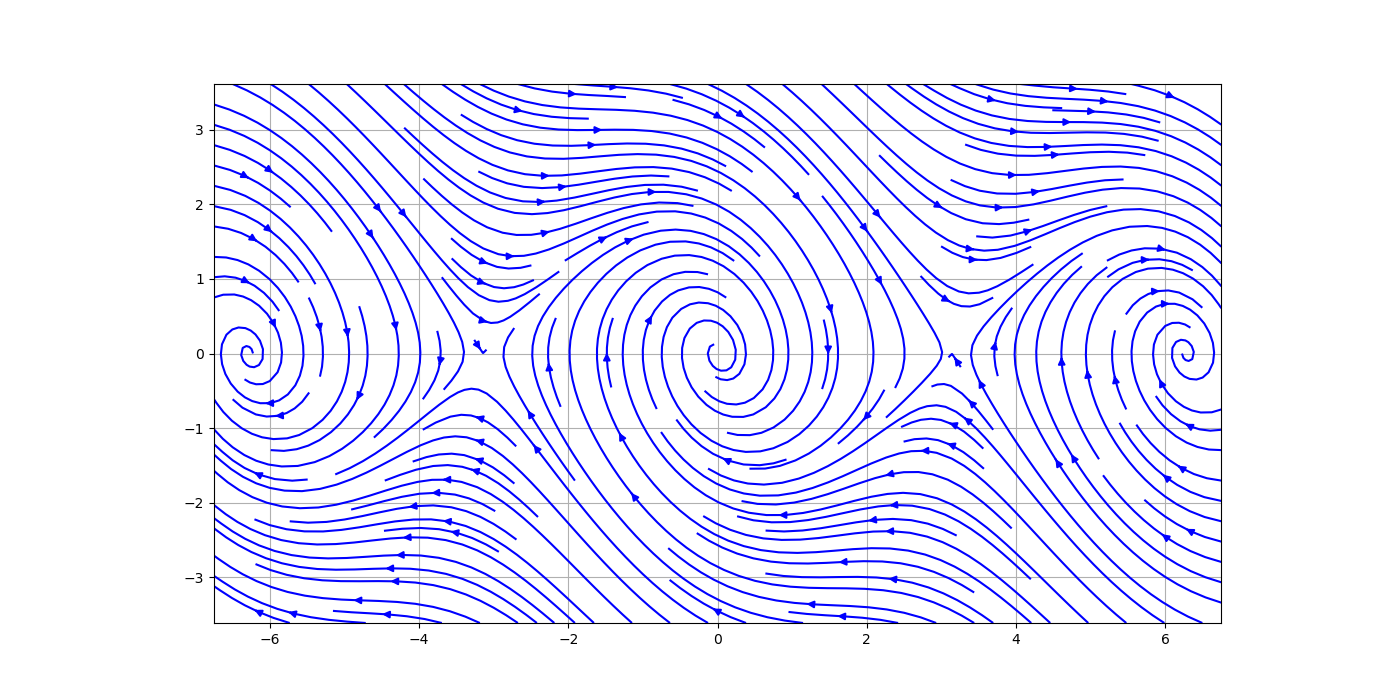
\includegraphics[width=0.5\textwidth]{images/hw_5/with_friction_0.4.png} &   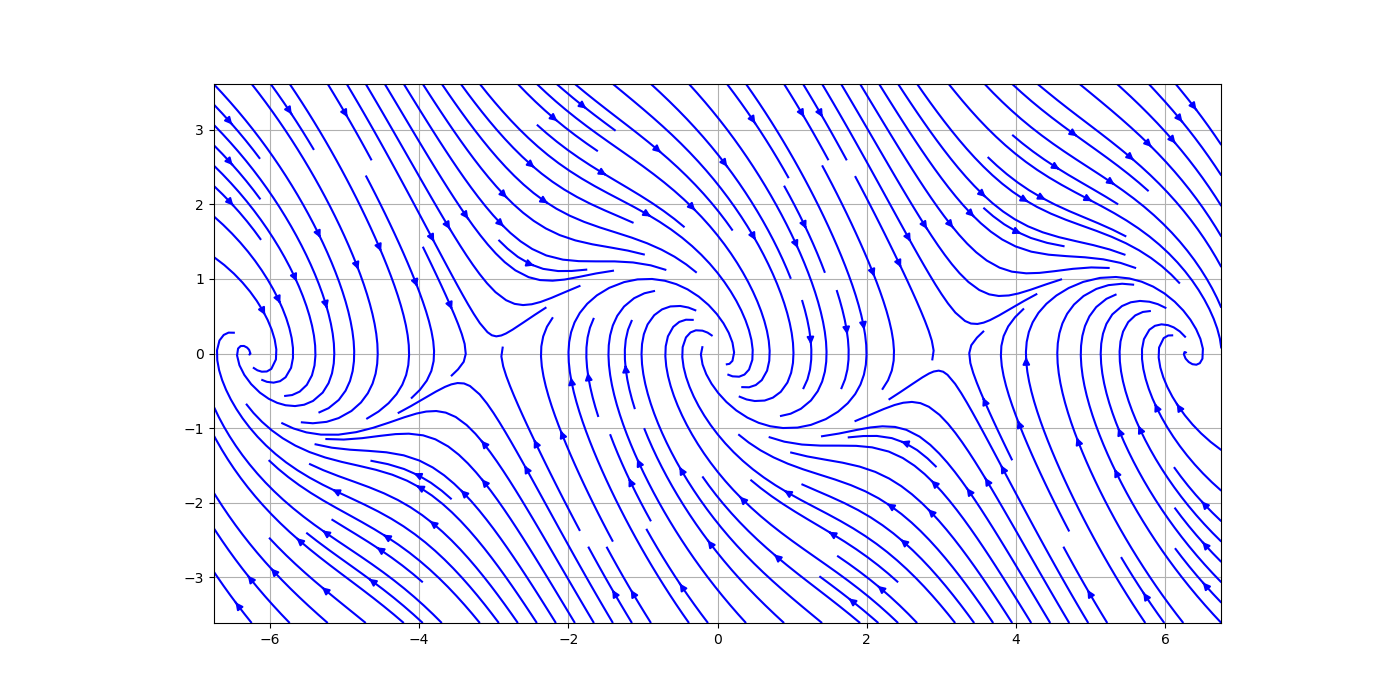
\includegraphics[width=0.5\textwidth]{images/hw_5/with_friction_1.png} \\
  $\kappa/\omega = 0.4$ & $\kappa/\omega = 1.0$ \\
  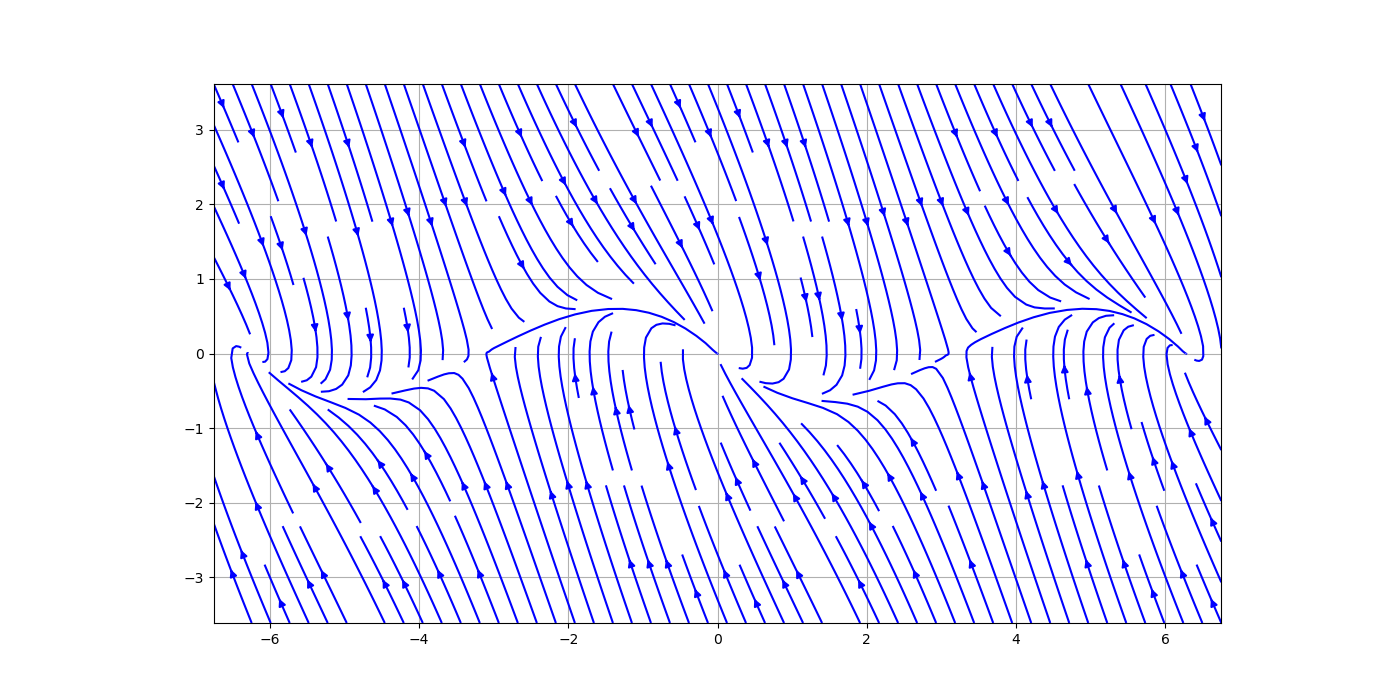
\includegraphics[width=0.5\textwidth]{images/hw_5/with_friction_2.png} &   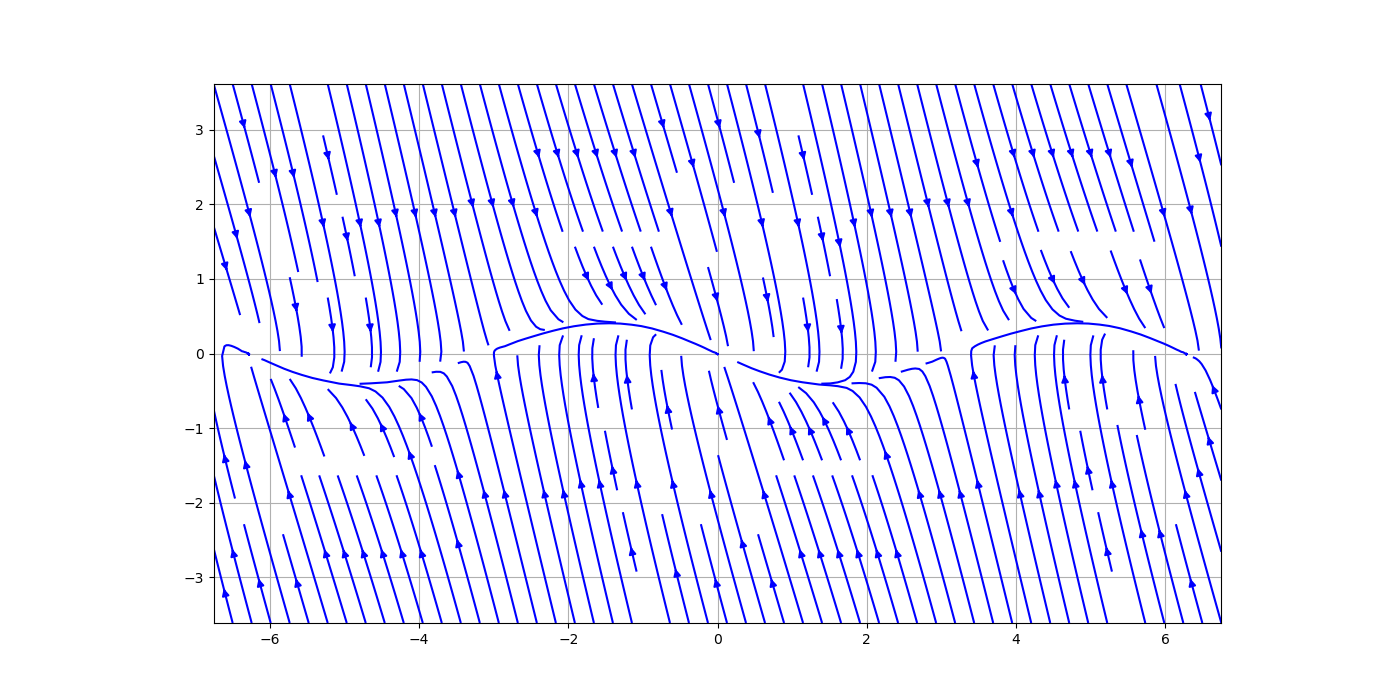
\includegraphics[width=0.5\textwidth]{images/hw_5/with_friction_3.png} \\
  $\kappa/\omega = 2.0$ & $\kappa/\omega = 3.0$
\end{tabular}
    \caption{Фазовий портрет для задачі 3 для різних співвідношень $\kappa/\omega$.}
    \label{fig:with_friction}
\end{figure}

\end{document}
